%%%%%%%%%%%%%%%%%%%%%%%%%%%%%%%%%%%%%%%%%%%%%%%%%%%%%%%%%%%%%%%%%%%
%% ACO-Adaptive Compute Scheduler
%% HiPC 2026 — IEEE International Conference on High Performance
%% Computing, Data, and Analytics
%% Track: AI Systems and Applications
%% Deadline: July 1, 2026
%%
%% DOUBLE-BLIND SUBMISSION: author/affiliation withheld
%%%%%%%%%%%%%%%%%%%%%%%%%%%%%%%%%%%%%%%%%%%%%%%%%%%%%%%%%%%%%%%%%%%

\documentclass[conference]{IEEEtran}
\IEEEoverridecommandlockouts

\usepackage{cite}
\usepackage{amsmath,amssymb,amsfonts}
\usepackage{graphicx}
\usepackage{textcomp}
\usepackage{xcolor}
\usepackage{booktabs}
\usepackage{float}
\usepackage{url}
\usepackage{tikz}
\usetikzlibrary{positioning}
\renewcommand{\ttdefault}{cmtt}

\begin{document}
\title{ACO-Adaptive Scheduling: Why Signal Design Outperforms\\
       Deep Learning Predictors in Heterogeneous Clusters}

% DOUBLE-BLIND: author block anonymised for submission
\author{
  \IEEEauthorblockN{Anonymous Author(s)}
  \IEEEauthorblockA{Affiliation withheld for double-blind review}
}

\maketitle

% =============================================================
\begin{abstract}
Production cluster schedulers for heterogeneous GPU and CPU workloads
face incompatible scheduling contracts: inference jobs cannot tolerate
queuing, batch actors checkpoint across preemption boundaries, and stream
processors shift CPU demand on sub-second timescales --- a combination
reactive orchestrators cannot serve without forward-looking utilization
signals. We present ACO-Adaptive, a centralized scheduler combining Ant
Colony Optimization with a pluggable per-node predictor module for
cost-aware, QoS-preserving job placement. The ACO colony accumulates
per-node pheromone trails across scheduling calls; predictor output enters
a multiplicative CostEngine heuristic that penalizes nodes forecast to
spike prior to placement. To identify the best predictor for this role, we
conduct a 14-way ablation (10 seeds $\times$ 200 latency-critical jobs,
32-node cluster) spanning deep-learning models (LSTM, GRU, TCN,
Transformer, MLP), classical time-series methods (ARIMA, linear
regression), and signal compression predictors (EMA, moving average,
persistence). Signal compression predictors lead: EMA~($\alpha{=}0.5$) achieves
\textbf{89.2\%} safe-node routing versus \textbf{75.4\%} for LSTM on
the CPU ablation testbed (\textbf{13.8\,pp} gap); a confirmatory
cross-section on 32 heterogeneous GPU nodes (7 types,
\$0.45--\$3.20/GPU-hr) widens this to \textbf{66.9\,pp}, with
freshly-initialized LSTM falling \textbf{26.4\,pp below} the
no-prediction baseline. A systematic sweep over effective memory horizon $H$
identifies a sharp optimum at $H^{*}{\approx}2.5$ ticks; past
$H{\approx}10$, over-smoothing inverts the spike signal entirely
(MA $w{=}30 \to 0.0\%$, EMA $\alpha{=}0.05 \to 0.0\%$). On
cluster-level metrics, ACO-Adaptive achieves 28.6\% cost reduction over
First-Fit on CPU workloads, 97.4\% QoS compliance on GPU workloads, and
P99 scheduling latency below 0.75\,ms across burst sizes from 1 to 200
concurrent jobs, scaling to 4.32\,ms P99 at 1{,}024 nodes.
\end{abstract}

\begin{IEEEkeywords}
cluster scheduling, ant colony optimization, signal compression, LSTM,
GPU scheduling, QoS, heterogeneous clusters, memory horizon
\end{IEEEkeywords}


% =============================================================
\section{Introduction}
% =============================================================

Inference, batch analytics, and stream-processing tasks run on shared
cluster hardware but impose contradictory scheduling contracts. An
inference job cannot queue at all; a batch actor checkpoints and resumes
across preemption boundaries; a stream processor shifts CPU demand faster
than a reactive scheduler can observe. Handling all three simultaneously
requires cost awareness (prefer cheaper nodes when quality constraints are
met), QoS discrimination (separate latency-sensitive from preemptible jobs
at placement time), and a forward utilization signal (avoid nodes whose
load will surge before the job finishes).

Production schedulers do not provide the third. Borg~\cite{verma2015borg},
Omega~\cite{schwarzkopf2013omega}, Mesos~\cite{hindman2011mesos}, and
YARN~\cite{vavilapalli2013yarn} consult observed resource availability at
decision time and carry no forward-looking utilization model;
Kubernetes~\cite{burns2016borg} adds configurable scoring plugins but
remains reactive. Min-cost flow schedulers such as
Firmament~\cite{gog2016firmament} achieve tight placement quality without
runtime load signals. Reinforcement learning approaches including
DeepRM~\cite{mao2016deeprm} and Decima~\cite{mao2019decima} learn strong
policies but depend on offline training corpora and degrade on
out-of-distribution workloads.

GPU-specialized schedulers such as Gandiva~\cite{xiao2018gandiva} and
Tiresias~\cite{gu2019tiresias} address fragmentation in deep learning
clusters but are purpose-built for homogeneous GPU pools and do not
generalize cost-aware placement across heterogeneous GPU tiers.

This paper presents \textbf{ACO-Adaptive}, a centralized cluster scheduler
addressing all three gaps through jointly operating components. Beyond the
scheduler itself, we ask a design question: \emph{which predictor class
best serves the routing task?} The 14-way ablation in
Section~\ref{subsec:comparison} answers it --- signal compression leads
every learned model by 13.8\,pp on the CPU testbed and 66.9\,pp on the
heterogeneous GPU topology (Section~\ref{subsec:gpu_confirm}).

This paper makes four contributions:
\begin{enumerate}
\item \textbf{A 14-way predictor ablation} showing that signal compression
      (EMA $\alpha{=}0.5$, Moving Average, Persistence) outperforms
      deep-learning predictors on the Alibaba 2018 cluster trace
      (low-to-moderate burst autocorrelation, 5-minute telemetry
      granularity), with EMA $\alpha{=}0.5$ leading at \textbf{89.2\%}
      versus \textbf{75.4\%} for LSTM ($+$\textbf{13.8\,pp}), at zero
      training cost and with no cold-start period. A confirmatory
      cross-section on 32 heterogeneous GPU nodes (7 types,
      \$0.45--\$3.20/GPU-hr) widens the gap to \textbf{66.9\,pp}:
      freshly-initialized LSTM inverts the routing signal, falling
      26.4\,pp \emph{below} the no-prediction baseline.
\item \textbf{An optimal memory horizon characterization
      ($H^{*}{\approx}2.5$)} showing a routing cliff beyond $H{\approx}10$
      where over-smoothing inverts the spike signal, collapsing routing to
      0\% for both MA ($w{=}30$) and EMA ($\alpha{=}0.05$). A LOOKBACK
      sweep (\texttt{LOOKBACK} $\in \{5,10,20,50\}$) confirms $H^*$ is
      stable near 2.5 for \texttt{LOOKBACK} $\in [10,50]$, indicating
      $H^*$ reflects workload burst structure, not our hyperparameter.
\item \textbf{A predictive placement architecture} combining ACO pheromone
      learning with a pluggable per-node predictor module, requiring no
      offline training phase. Any class implementing
      \texttt{fit}/\texttt{predict} can be substituted at runtime.
\item \textbf{An intent-based QoS routing layer} that enforces tier-specific
      scheduling strategies (ON\_DEMAND preference, fast-path bypass)
      achieving \textbf{97.4\%} LS$\to$ON\_DEMAND compliance on Alibaba
      GPU cluster traces.
\end{enumerate}


% =============================================================
\section{Related Work}
% =============================================================

\subsection{Production Cluster Schedulers}

Borg~\cite{verma2015borg} manages Google's production clusters using a
centralized Borgmaster with feasibility and scoring functions.
Omega~\cite{schwarzkopf2013omega} extends this with shared-state optimistic
concurrency. Both systems prioritize stability over cost optimization and
lack predictive utilization models. Mesos~\cite{hindman2011mesos} delegates
placement to framework schedulers via resource offers;
YARN~\cite{vavilapalli2013yarn} follows a similar delegation model. All
four share a limitation acknowledged in the Borg
retrospective~\cite{burns2016borg}: scheduling decisions are reactive,
taken on observed state without anticipating near-term utilization changes.

\subsection{Cost- and Quality-Aware Scheduling}

Firmament~\cite{gog2016firmament} formulates scheduling as min-cost
max-flow over a preference graph, achieving sub-100\,ms latency for large
clusters. Tetris~\cite{grandl2014tetris} uses a dot-product alignment score
to pack multiple resource dimensions simultaneously; its composite scoring
philosophy directly inspired our CostEngine design.
Paragon~\cite{delimitrou2013paragon} and
Quasar~\cite{delimitrou2014quasar} use QoS-aware classification to improve
placement in heterogeneous clusters, a concept extended through our
WorkloadIntentRouter.
Sparrow~\cite{ousterhout2013sparrow} targets $<$100\,\textmu{}s latency
via distributed sampling, trading placement quality for speed.

\subsection{Reinforcement Learning Schedulers}

DeepRM~\cite{mao2016deeprm} trains a deep network to minimize job slowdown.
Decima~\cite{mao2019decima} uses a graph neural network trained on the
Alibaba cluster trace to learn DAG-aware scheduling policies. Both require
an offline training phase. ACO-Adaptive differs: pheromone learning is
online and continuous, requires no pre-training, and the influence of each
preference is directly interpretable from the pheromone vector.

\subsection{GPU Cluster Schedulers}

Gandiva~\cite{xiao2018gandiva} addresses head-of-line blocking via GPU
time-slicing and migration. Tiresias~\cite{gu2019tiresias} schedules
distributed DL jobs using Least Attained Service. The Alibaba GPU cluster
trace used in our evaluation was introduced by Weng et
al.~\cite{weng2023beware}, who additionally propose Fragmentation Gradient
Descent as a GPU allocation strategy. ACO-Adaptive complements these
systems by targeting cost-aware, QoS-discriminating placement across
heterogeneous GPU node tiers rather than scheduling within a homogeneous
pool.

\subsection{Ant Colony Optimization}

The ACO metaheuristic was introduced by Dorigo and
Gambardella~\cite{dorigo1997ant}; the foundational treatment of parameter
selection is given in~\cite{dorigo2004aco}. Our colony follows Ant Colony
System (ACS) conventions: $\alpha{=}1.0$, $\beta{=}2.0$, $\rho{=}0.1$,
20 ants per cycle, 5 iterations, early stopping at stagnation limit 3.

\subsection{Time-Series Prediction in Scheduling}

Time-series forecasting has been studied in cloud autoscaling and capacity
planning. Roy et al.~\cite{roy2011autoscaling} demonstrate ARIMA-based
workload forecasting for elastic cloud provisioning; Cortez et
al.~\cite{cortez2017resource} apply neural-network prediction to
Azure VM workload traces for capacity management; Rzadca et
al.~\cite{rzadca2020autopilot} describe Google Autopilot, which uses
exponential smoothing for resource recommendation in production.
Tsafrir et al.~\cite{tsafrir2007backfill} show that simple system-generated
predictions (recent-job-average) outperform user-supplied runtime estimates
for HPC backfill scheduling --- an early analogue of our finding.

These works use prediction as a \emph{quantitative capacity estimate}.
ACO-Adaptive uses prediction as a binary \emph{routing signal}: the output
is a spike probability that gates node selection, not a capacity quantity.
Under this formulation, the directional accuracy of the signal above a
placement threshold matters more than numeric forecast precision. Our 14-way
ablation tests this distinction directly across four predictor classes.
That signal compression at $H^{*}{\approx}2.5$ leads every learned model
is consistent with Tsafrir et al.'s observation that simpler predictors
can outperform complex ones when the signal structure is exploited
correctly~\cite{tsafrir2007backfill}.

\subsection{Positioning Relative to Production Schedulers}

ACO-Adaptive acts as a predictive placement layer extending default
scheduling logic by incorporating forward-looking utilization signals and
historical placement preferences into a unified cost-aware scoring
function. A Kubernetes deployment with a custom \texttt{NodeResourcesFit}
scoring plugin could approximate the CostEngine for cost-only objectives,
but kube-scheduler is stateless and purely reactive: it has no mechanism
to (i) incorporate predictor-based load forecasts, (ii) learn per-node
preferences from placement outcomes, or (iii) enforce structured QoS tier
policies without heavyweight admission controllers. ACO-Adaptive's
pheromone mechanism provides a lightweight online alternative without
requiring external metrics infrastructure or custom admission webhooks.


% =============================================================
\section{System Design}
% =============================================================

ACO-Adaptive is a centralized scheduler implemented in Python with a
FastAPI REST interface. Figure~\ref{fig:arch} shows the top-level
architecture. Five components form the control plane; a NodeAgent layer
constitutes the data plane.

\begin{figure*}[t]
\centering
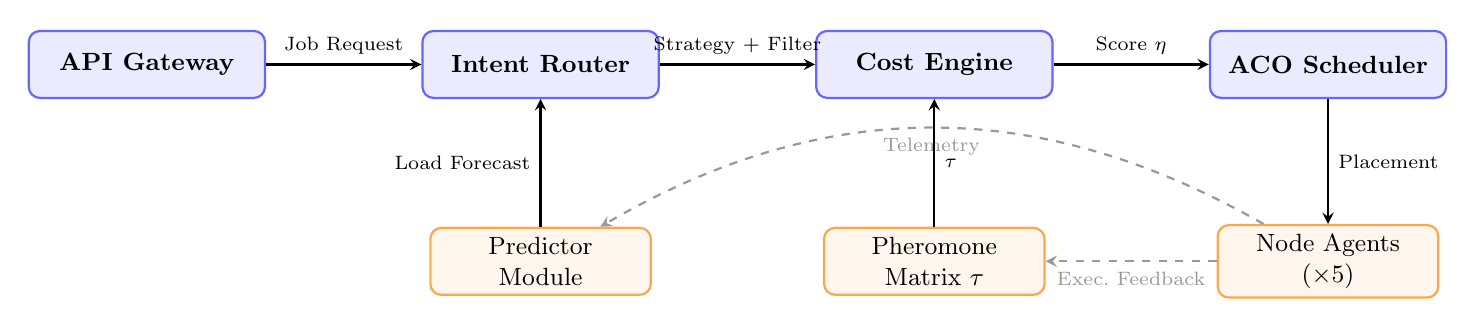
\begin{tikzpicture}[>=stealth, thick]
  \tikzstyle{cbox}=[rectangle, draw=blue!60, fill=blue!8, rounded corners=4pt,
                    minimum width=3.0cm, minimum height=0.85cm,
                    align=center, font=\small\bfseries]
  \tikzstyle{sbox}=[rectangle, draw=orange!70, fill=orange!7, rounded corners=4pt,
                    minimum width=2.8cm, minimum height=0.85cm,
                    align=center, font=\small]
  \tikzstyle{arr}=[->, thick, >=stealth]
  \tikzstyle{darr}=[->, thick, dashed, >=stealth, gray!80]

  \node[cbox] at ( 1.5, 0) (api)    {API Gateway};
  \node[cbox] at ( 6.5, 0) (router) {Intent Router};
  \node[cbox] at (11.5, 0) (cost)   {Cost Engine};
  \node[cbox] at (16.5, 0) (aco)    {ACO Scheduler};

  \node[sbox] at ( 6.5,-2.5) (pred)  {Predictor\\Module};
  \node[sbox] at (11.5,-2.5) (phero) {Pheromone\\Matrix $\tau$};
  \node[sbox] at (16.5,-2.5) (agents){Node Agents\\($\times$5)};

  \draw[arr] (api)    -- node[above, font=\scriptsize]{Job Request}       (router);
  \draw[arr] (router) -- node[above, font=\scriptsize]{Strategy + Filter} (cost);
  \draw[arr] (cost)   -- node[above, font=\scriptsize]{Score $\eta$}      (aco);
  \draw[arr] (aco)    -- node[right, font=\scriptsize]{Placement}         (agents);

  \draw[darr] (agents) to[bend right=30]
              node[below, font=\scriptsize, pos=0.5]{Telemetry} (pred);
  \draw[darr] (agents) --
              node[below, font=\scriptsize]{Exec.\ Feedback} (phero);

  \draw[arr] (pred)  -- node[left,  font=\scriptsize]{Load Forecast} (router);
  \draw[arr] (phero) -- node[right, font=\scriptsize]{$\tau$}        (cost);
\end{tikzpicture}
\caption{ACO-Adaptive system architecture. Solid arrows: synchronous
scheduling path. Dashed arrows: asynchronous feedback --- Node Agents
stream telemetry to the Predictor Module and report execution outcomes
to the Pheromone Matrix.}
\label{fig:arch}
\end{figure*}

\subsection{ACO Colony Engine}

The scheduler models the set of healthy cluster nodes as the ACO decision
graph. Each node $n_i$ carries a pheromone value $\tau_i \geq \tau_{\min}$
that accumulates over successful placements and evaporates over time.
At each scheduling call a colony of $k{=}20$ ants independently selects a
node using:

\begin{equation}
  P(n_i \mid j) = \frac{\tau_i^{\alpha} \cdot \eta_i^{\beta}}
                       {\sum_{n_\ell \in \mathcal{F}(j)}
                        \tau_\ell^{\alpha} \cdot \eta_\ell^{\beta}}
  \label{eq:aco}
\end{equation}

where $\mathcal{F}(j)$ is the feasible set for job $j$,
$\alpha{=}1.0$ controls pheromone influence, $\beta{=}2.0$ controls
heuristic influence, and $\eta_i$ is the composite cost-engine score for
node $n_i$. Pheromone is updated with a flat deposit
$\Delta\tau_i = Q = 1.0$ on the selected node and global evaporation:
$\tau_i \leftarrow \text{clip}((1{-}\rho)\tau_i,\;\tau_{\min},\;\tau_{\max})$
with $\rho{=}0.1$, $\tau_{\min}{=}0.01$, $\tau_{\max}{=}10.0$.
With $A{=}20$, $I{=}5$, and early stopping at stagnation limit 3,
placement completes in sub-millisecond time
(Section~\ref{subsec:latency}).

\subsection{Cost Engine}

The cost-engine heuristic $\eta_i$ for node $n_i$ is a multiplicative
composite of four sub-scores, each in $(0,1]$:

\begin{equation}
  \eta_i = r_i \cdot c_i \cdot s_i \cdot p_i
  \label{eq:cost}
\end{equation}

where $r_i$ is a reliability factor penalizing SPOT interruption
probability; $c_i$ is an asymptotic inverse cost factor
($1 / (1 + \text{norm\_cost})$); $s_i$ is an SLA headroom factor
($(100 - \text{cpu\_util\%})/100$, strict for LATENCY\_CRITICAL, floored
at 0.1 for BATCH); and $p_i$ is the prediction factor from the Predictor
Module. A score of $\eta_i = 0$ is a hard gate --- the node is never
selected regardless of pheromone strength.

The prediction factor $p_i$ is a monotonic heuristic penalty that
decreases as the one-step forecast $\hat{u}_i$ rises above the node's
recent mean $\bar{u}_i$ (mean over \texttt{LOOKBACK=10} ticks):
\begin{equation}
  p_i = 1 - \Bigl(\max\!\bigl(0,\;(\hat{u}_i - \bar{u}_i)/\bar{u}_i\bigr)
               \cdot w \cdot c_{\text{conf}}\Bigr)
  \label{eq:pi}
\end{equation}
where $w{=}0.5$ is the spike penalty weight and $c_{\text{conf}} \in [0,1]$
is predictor confidence. As $\hat{u}_i$ rises above $\bar{u}_i$, $p_i$
falls monotonically; when no prediction is available, $p_i = 1.0$
(neutral).

\subsection{Predictor Module}

The Predictor Module provides per-node one-step CPU utilization forecasts
for the CostEngine's $p_i$ factor. It exposes a two-method interface:

\begin{itemize}
  \item \texttt{fit(profile)} --- update internal state from the node's
        recent utilization history
  \item \texttt{predict(profile)} --- return a one-step forecast and a
        confidence score $c_{\text{conf}} \in [0,1]$
\end{itemize}

Any class implementing this interface can serve as the per-node predictor;
the module is swapped at runtime without restarting the scheduler. The
scheduler is predictor-agnostic: it consumes only the forecast value and
confidence score, not the predictor's internal representation.

The default implementation ships an LSTM~\cite{hochreiter1997lstm}; the
ablation and compression sweep evaluated in
Sections~\ref{subsec:comparison}--\ref{subsec:hstar} show that
EMA $\alpha \in [0.4, 0.7]$ outperforms it by 13.8\,pp.
Implementation details for all 14 evaluated predictors are given in
Section~\ref{subsec:roster}.

\subsection{Workload Intent Router}

The WorkloadIntentRouter classifies incoming jobs into
\texttt{LATENCY\_CRITICAL}, \texttt{BATCH}, or \texttt{STREAM\_PROCESSING}
tiers based on declared QoS parameters. Each tier maps to a
SchedulingStrategy configuring CostEngine weights, instance-type
preferences, and routing behavior. Latency-critical jobs receive
ON\_DEMAND preference and bypass the full colony iteration via a
single-pass argmax over the feasible node set; this fast path is triggered
by QoS tier classification, not by a runtime confidence threshold. Batch
jobs accept SPOT nodes and permit preemption. QoS mapping follows the
Alibaba GPU cluster trace~\cite{weng2023beware} (LS $\to$
\texttt{LATENCY\_CRITICAL}, BE $\to$ \texttt{BATCH}).

\subsection{Telemetry Collector and Trace Adapter}

The TelemetryCollector runs a per-node tick loop sampling CPU and memory
utilization, updating node state, and accumulating WorkloadProfiles for
predictor training. A pluggable trace adapter interface allows replaying
production telemetry in place of live measurements. The
AlibabaMachineTraceAdapter replays the Alibaba 2018 cluster
trace~\cite{alibaba2018trace} with per-node time offsets and scale factors
to produce differentiated utilization profiles.

\subsection{Node Agent and REST API}

The NodeAgent constitutes the data plane, simulating job execution with
configurable duration and resource release semantics. The REST API exposes
\texttt{POST /jobs}, \texttt{GET /nodes}, \texttt{GET /metrics}, and
\texttt{GET /predict/:node\_id} endpoints, along with
\texttt{POST /upload-trace} for hot-swapping the trace adapter at runtime.
A built-in HTML dashboard polls the API every three seconds, displaying
node utilization, predictor confidence, and live job status.


% =============================================================
\section{Experimental Setup}
% =============================================================

\subsection{Cluster Topologies}

We evaluate on three topologies. The \emph{balanced CPU topology} consists
of three node classes: a mid-tier ON\_DEMAND node at \$0.70/hr, a premium
ON\_DEMAND node at \$1.00/hr, and a SPOT node at \$0.50/hr, each with
64 cores and 256\,GB memory. The \emph{GPU topology} is sampled from real
Alibaba production hardware: 32 nodes spanning seven GPU models (A10, G2,
G3, P100, T4, V100M16, V100M32) with per-node costs ranging from
\$0.60/hr to \$25.60/hr. For predictor ablation and signal compression
experiments (Sections~\ref{subsec:calibration}--\ref{subsec:hstar}), we
use a \emph{32-node predictor testbed} of identically priced ON\_DEMAND
nodes (\$0.80/hr, 32 cores, 64\,GB), so that the only differentiator in
$\eta_i$ is the prediction factor $p_i$. For scalability experiments
(Section~\ref{subsec:scalability}), synthetic heterogeneous clusters from
32 to 1{,}024 nodes are generated (60\% ON\_DEMAND x86\_64, 25\% SPOT
ARM64, 15\% ON\_DEMAND GPU).

\subsection{Workload Traces}

\textbf{Azure VM Trace.} Job CPU core counts are drawn from the
AzureTracesForPacking2020 dataset~\cite{hadary2020protean} (114 million VM
allocation requests), yielding a bimodal distribution peaking at 2 cores
(45\%) and 8 cores (24\%).

\textbf{Alibaba 2018 Machine Trace.} Utilization data is sourced from
cluster-trace-v2018~\cite{alibaba2018trace}, a 2{,}243-row trace at
5-minute granularity over eight days.\footnote{The Alibaba trace provides
an aggregate cluster signal. Per-node diversity in the testbed is produced
by applying time-windowed offsets to this signal for each node.} For the
32-node predictor testbed, 32 non-overlapping 100-row windows are selected
via a dense candidate search (stride\,=\,10 rows) ranked by
$\text{score} = \sigma_w + \max(\text{tail\_rise},\, 0)$, where
tail\_rise is the mean CPU difference between the last 10 and prior 20
rows (aligned with \texttt{LOOKBACK=10}). The 16 lowest-scoring windows
form the \emph{stable group} (mean 39.5\%\,CPU, $\sigma{=}5.8\%$,
declining tail) and the 16 highest form the \emph{volatile group}
(mean 39.5\%\,CPU, $\sigma{=}8.6\%$, rising tail,
$\overline{\text{tail\_rise}}{=}{+}7.7$\,pp).

\textbf{Alibaba GPU Trace (ATC'23).} GPU workloads are from the OpenB
dataset~\cite{weng2023beware}: 4{,}334 usable tasks from 1{,}213 GPU
nodes; 1{,}517 carry explicit GPU model constraints. A stratified sample
of 100 jobs preserving the LS/BE ratio (78\%/22\%) is used per run.

\subsection{Scheduling Baselines}

\textit{First-Fit} selects the first healthy node satisfying all resource
constraints~\cite{verma2015borg}. \textit{Random} selects uniformly from
the feasible set. \textit{Tetris}~\cite{grandl2014tetris} selects the node
maximizing $\sum_k (J_k/C_k)(A_k/C_k)$ across CPU, memory, and GPU
dimensions.

\subsection{Predictor Implementations}
\label{subsec:roster}

\textbf{Default (LSTM).} Single-layer LSTM~\cite{hochreiter1997lstm},
hidden size 32, \texttt{num\_layers=1}, trained with Adam on a sliding
window of \texttt{LOOKBACK=10} ticks, refitted asynchronously every ten
telemetry ticks. Confidence initializes at 0.1 on cold start ($p_i = 1.0$),
crossing the 0.3 meaningful-signal threshold at 50--100 ticks
(4.2--8.3 hours at 5-minute Alibaba granularity).

\textbf{Deep learning.} GRU (hidden 32), MLP (hidden 32, 2 layers),
TCN (causal Conv1d, kernel\,=\,3, hidden 32), Transformer (encoder,
$d_{\text{model}}{=}32$, 4 heads) --- all PyTorch, same sliding window
and Adam configuration as the default LSTM.

\textbf{Classical ML.} Linear Regression (OLS on $z$-scored lag window),
ARIMA(1,0,1) and ARIMA(1,1,1) (statsmodels).

\textbf{Signal compression.} EMA ($\alpha \in \{0.1, 0.3, 0.5\}$),
Moving Average ($w{=}5$), Persistence (last observed value). No training
or warm-up required; available from the first telemetry tick.

\textbf{14-way ablation protocol (Section~\ref{subsec:comparison}).}
10 seeds $\times$ 200 LC jobs per predictor on the 32-node predictor
testbed.

\textbf{Signal compression sweep (Section~\ref{subsec:hstar}).}
MA $w \in \{1,2,3,5,7,10,15,20,30,50\}$;
EMA $\alpha \in \{0.05, 0.10, 0.15, 0.20, 0.30, 0.40, 0.50, \ldots, 1.00\}$.
Unified effective memory horizon: $H_{\text{MA}} = (w{+}1)/2$,
$H_{\text{EMA}} = 1/\alpha$. Metrics: routing\%, Spearman
$\rho$(predicted spike probability, true node volatility), Top-10 accuracy.

\textbf{LOOKBACK sensitivity sweep.} Repeats the EMA sweep above for
\texttt{LOOKBACK} $\in \{5, 10, 20, 50\}$ to characterize $H^*$
stability across prediction window sizes.

\textbf{Cross-topology GPU confirmation (Section~\ref{subsec:gpu_confirm}).}
Six-predictor cross-section (EMA $\alpha{=}0.5$, Persistence, No
prediction, GRU, TCN, LSTM) repeated on the 32-node GPU heterogeneous
topology (7 GPU models, \$0.45--\$3.20/GPU-hr). Deep-learning models
freshly initialized per seed (50 epochs, 90 training samples per node).

\textbf{ACO colony ablation.} Four-condition 2$\times$2 design (pheromone
$\times$ EMA): greedy-only, ACO-only, Greedy+EMA, ACO+EMA
(10 seeds $\times$ 200 LC jobs each).


% =============================================================
\section{Evaluation}
\label{sec:eval}
% =============================================================

\subsection{Predictor Signal Calibration}
\label{subsec:calibration}

Before comparing predictors we ask whether the signal is meaningful at all.
Figure~\ref{fig:lstm_cal} shows the default LSTM predictor's calibration
on the Alibaba 2018 machine trace (2{,}243 raw rows; 2{,}233
prediction--observation pairs after LOOKBACK warm-up).

\begin{figure}[t]
\centering
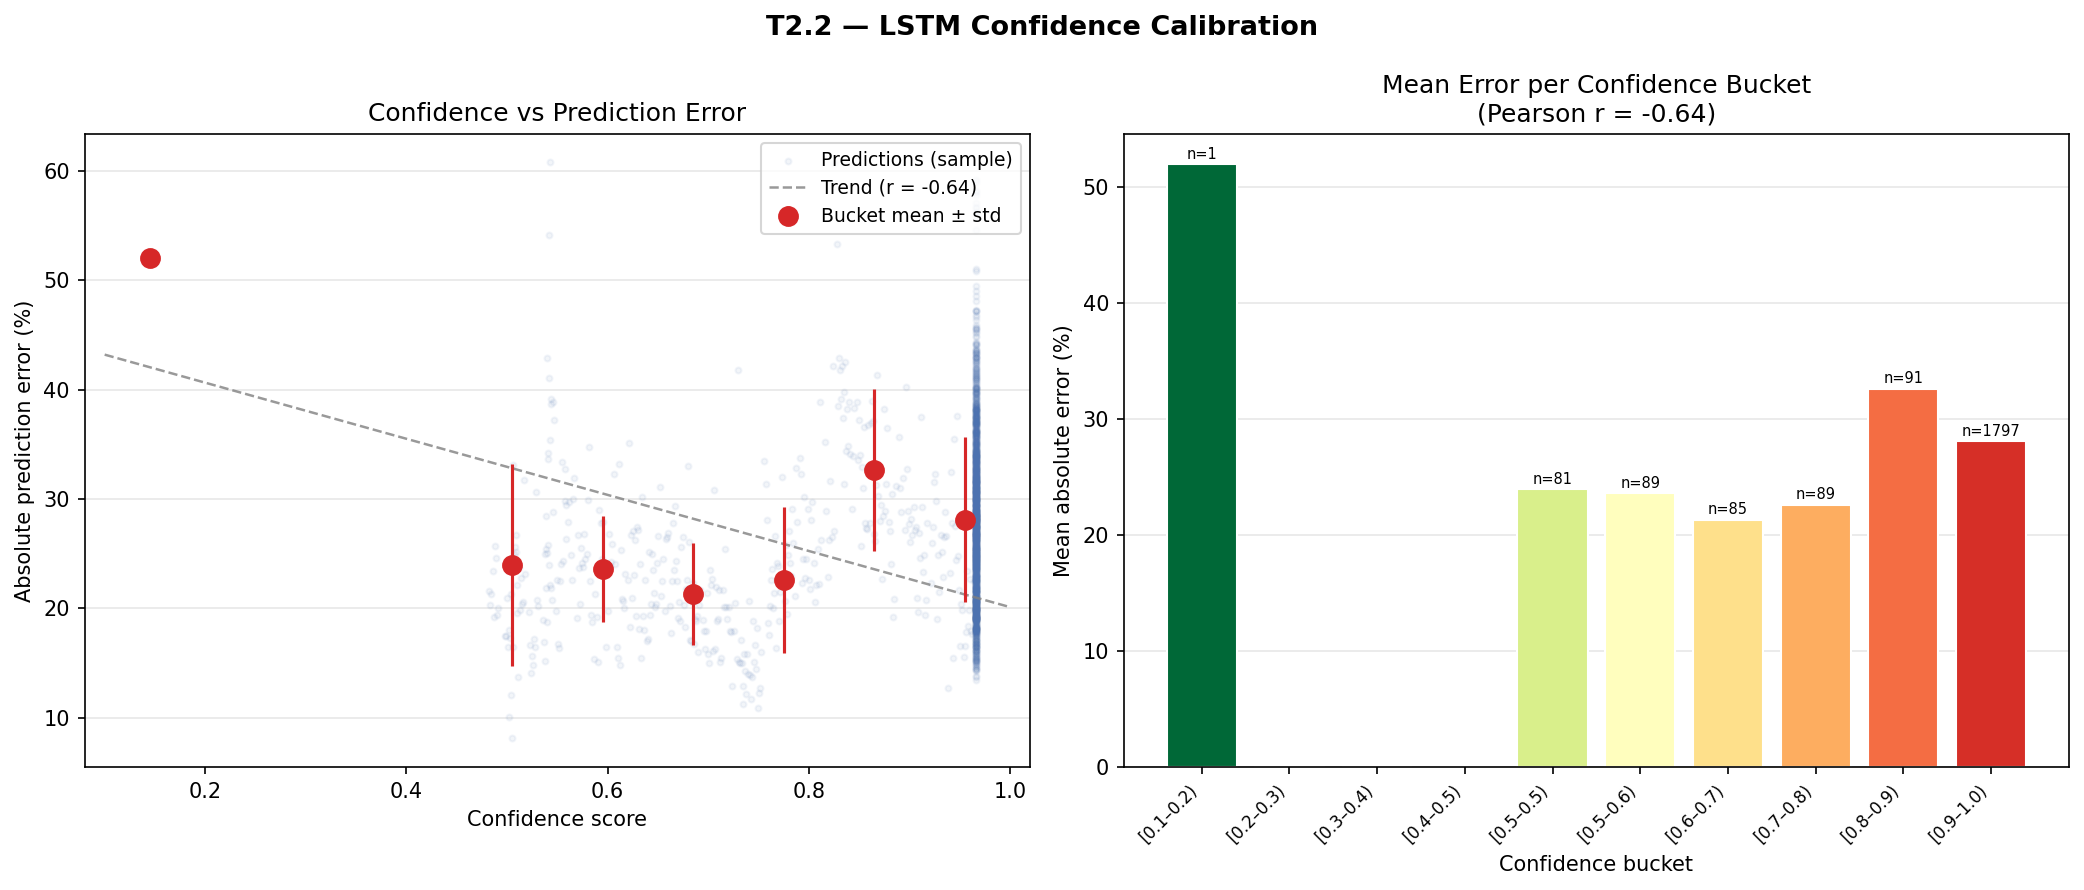
\includegraphics[width=\columnwidth]{figures/tier2_confidence_calibration.png}
\caption{Predictor calibration on the Alibaba 2018 trace. Higher predicted
utilization correlates with lower observed idle capacity
($r{=}{-}0.64$, $n{=}2{,}233$ pairs).}
\label{fig:lstm_cal}
\end{figure}

The Pearson correlation between predicted utilization and observed idle
capacity is $r = -0.64$ ($n{=}2{,}233$): nodes the predictor identifies
as loaded do have less idle capacity in practice. Spike recall on
the trace is 0/5 (0\%) at threshold 0.4 --- spikes are infrequent and
the predictor detects elevated baseline rather than onset timing. The
directional signal is real; the question is which predictor carries it
most effectively for routing decisions.

On the 32-node predictor testbed ($N{=}5$ seeds, 200 LC jobs per seed),
LSTM predictions raise stable-group placement from $48.8\%{\pm}3.9\%$
(no prediction, indistinguishable from random) to $80.3\%{\pm}3.2\%$ ---
a $+31.5$\,pp improvement ($t{=}22.56$, $p{<}0.001$, $df{=}4$). The
signal is non-trivial. Section~\ref{subsec:comparison} shows whether a
better predictor can do more with it.

\subsection{14-Way Predictor Comparison}
\label{subsec:comparison}

Figure~\ref{fig:ablation} shows routing\% for all 14 predictors.

\begin{figure}[t]
\centering
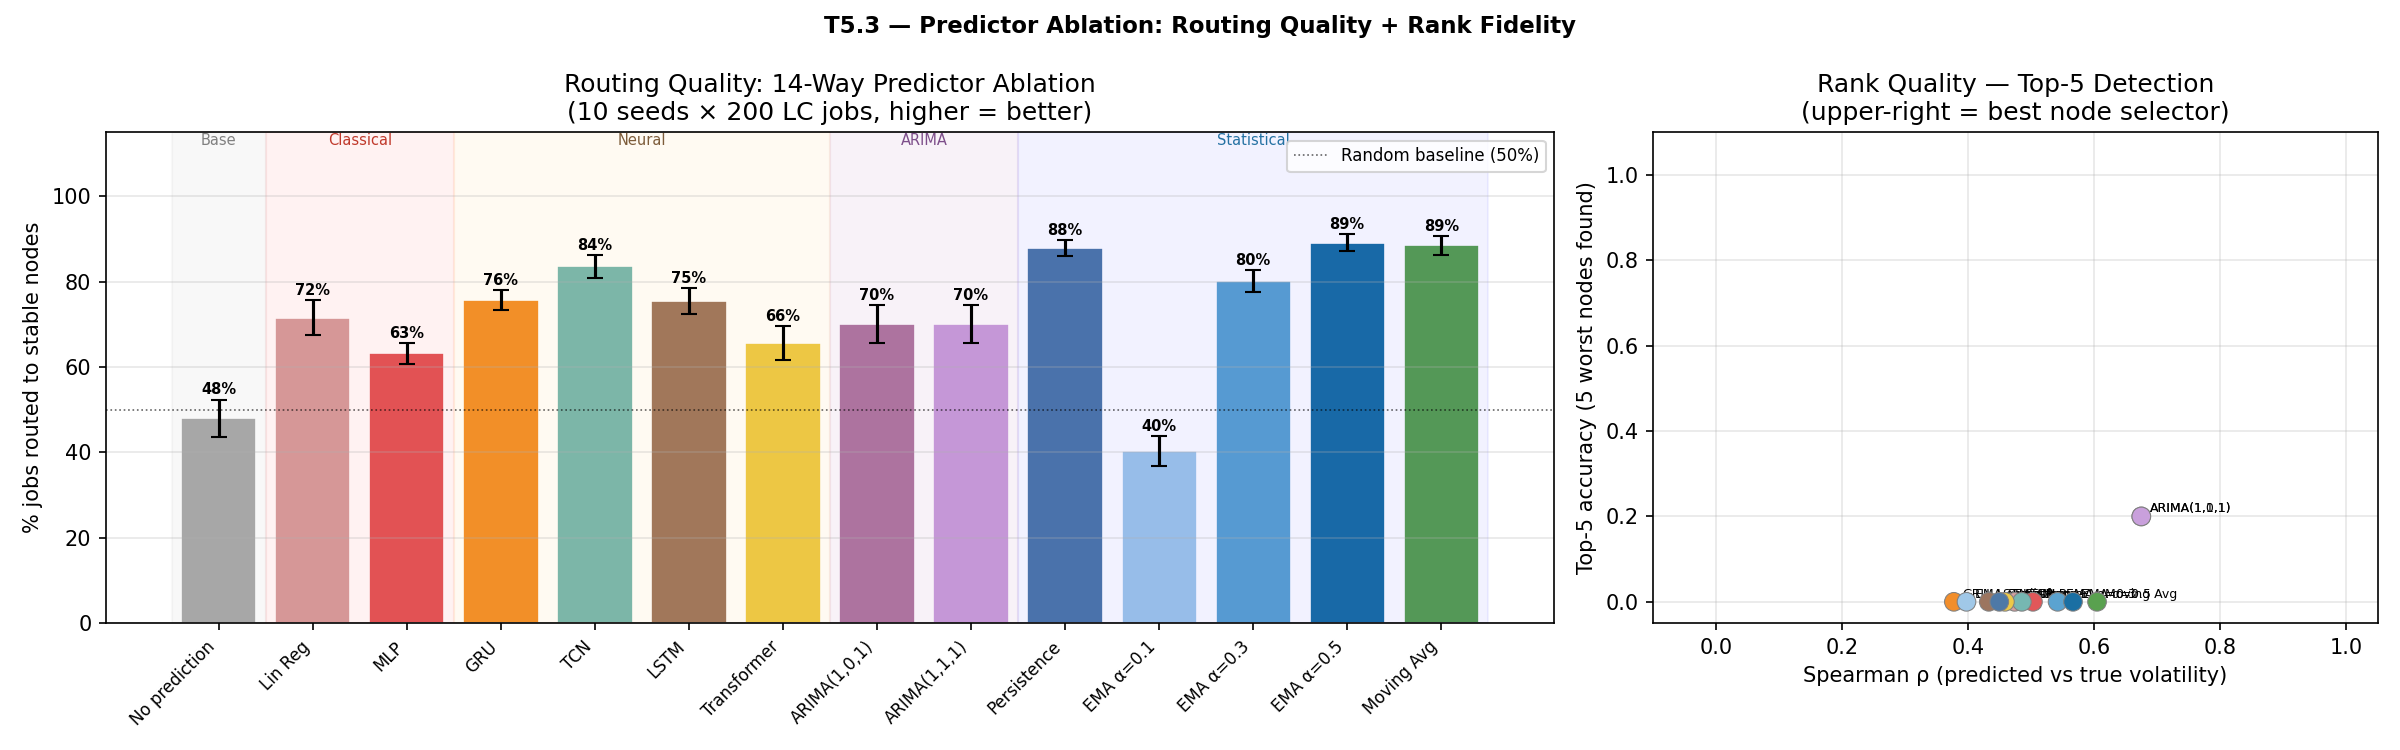
\includegraphics[width=\columnwidth]{figures/tier5_predictor_ablation.png}
\caption{14-way predictor ablation: routing\% to stable nodes
(10 seeds $\times$ 200 LC jobs). Signal compression predictors (top)
uniformly outperform deep-learning models (middle). EMA $\alpha{=}0.1$
collapses below random due to over-smoothing.}
\label{fig:ablation}
\end{figure}

\begin{table}[t]
\caption{14-way predictor ablation: routing\% to stable nodes
(mean$\pm$std, 10 seeds $\times$ 200 LC jobs; sorted descending).
Random baseline $\approx$50\%.}
\label{tab:ablation}
\begin{center}
\resizebox{\columnwidth}{!}{%
\begin{tabular}{llrr}
\toprule
\textbf{Predictor} & \textbf{Category} & \textbf{Routing (\%)}
  & \textbf{Spearman $\rho$} \\
\midrule
EMA $\alpha{=}0.5$   & Signal Comp. & $\mathbf{89.2 \pm 1.9}$ & 0.566 \\
Moving Avg ($w{=}5$) & Signal Comp. & $88.5 \pm 2.2$ & 0.605 \\
Persistence          & Signal Comp. & $87.8 \pm 1.9$ & 0.449 \\
TCN                  & Deep Learning & $83.6 \pm 2.7$ & 0.485 \\
EMA $\alpha{=}0.3$   & Signal Comp. & $80.1 \pm 2.6$ & 0.542 \\
GRU                  & Deep Learning & $75.7 \pm 2.4$ & 0.377 \\
LSTM                 & Deep Learning & $75.4 \pm 3.0$ & 0.433 \\
Lin Reg              & Classical ML  & $71.5 \pm 4.1$ & 0.474 \\
ARIMA(1,0,1)         & Classical ML  & $70.0 \pm 4.4$ & \textbf{0.675} \\
ARIMA(1,1,1)         & Classical ML  & $70.0 \pm 4.4$ & \textbf{0.675} \\
Transformer          & Deep Learning & $65.6 \pm 4.0$ & 0.458 \\
MLP                  & Deep Learning & $63.2 \pm 2.4$ & 0.503 \\
No prediction        & Baseline      & $48.0 \pm 4.3$ & --- \\
EMA $\alpha{=}0.1$   & Signal Comp.  & $40.3 \pm 3.6$ & 0.397 \\
\bottomrule
\end{tabular}}
\end{center}
\end{table}

Three patterns hold across all 10 seeds.

\textbf{Signal compression leads.} EMA~($\alpha{=}0.5$), Moving Average
($w{=}5$), and Persistence occupy the top three positions, all reaching
87--89\% routing. None require training, a warm-up period, or GPU
resources. EMA~($\alpha{=}0.5$) leads at \textbf{89.2\%}, beating LSTM
by \textbf{13.8\,pp}.

\textbf{Deep learning underperforms across all architectures.}
LSTM achieves 75.4\%, GRU 75.7\%, TCN 83.6\%, Transformer 65.6\%,
MLP 63.2\%. TCN is the strongest deep-learning predictor but still
5.6\,pp below EMA~($\alpha{=}0.5$). ARIMA(1,0,1) and ARIMA(1,1,1) produce
identical routing (70.0\%), confirming that differencing ($d{=}1$) is
neutral on the stationary 100-sample Alibaba windows.

\textbf{EMA~($\alpha{=}0.1$) inverts the signal.} At 40.3\% routing ---
worse than the no-prediction baseline (48.0\%) --- EMA ($\alpha{=}0.1$)
is the weakest non-trivial predictor. With $H{=}1/0.1{=}10$, the EMA
converges toward the global node mean, losing the directional spike signal.
All 25/25 seeds across the extended stability run fall below 50\%.

\textbf{Rank quality does not predict routing performance.} ARIMA produces
the highest Spearman $\rho{=}0.675$ yet achieves only 70.0\% routing ---
well below EMA~($\alpha{=}0.5$, $\rho{=}0.566$, routing 89.2\%). The
routing task is a nonlinear thresholded decision: argmax over 32 nodes
rewards directional signal clarity above the spike threshold, not numeric
forecast precision.

\subsection{Cross-Topology Confirmation: GPU Heterogeneous Cluster}
\label{subsec:gpu_confirm}

The 14-way ablation ran on identically priced nodes to isolate predictor
signal quality. To test whether the EMA advantage holds on genuinely
heterogeneous infrastructure, we repeated a six-predictor cross-section
on the 32-node GPU topology (7 GPU types, \$0.45--\$3.20/GPU-hr).
Deep-learning models were freshly initialized per seed (50 epochs,
90 training samples per node).

\begin{table}[t]
\caption{Cross-topology confirmatory ablation: routing\% on the
heterogeneous GPU topology (7 GPU types, \$0.45--\$3.20/GPU-hr).
Deep-learning models freshly initialized per seed.}
\label{tab:gpu_confirm}
\begin{center}
\begin{tabular}{lrr}
\toprule
\textbf{Predictor} & \textbf{Routing (\%)} & \textbf{Std} \\
\midrule
EMA $\alpha{=}0.5$    & $\mathbf{100.0}$ & 0.0 \\
Persistence            & $\mathbf{100.0}$ & 0.0 \\
No prediction          &            59.5  & 3.6 \\
GRU (retrained/seed)   &            35.7  & 6.0 \\
TCN (retrained/seed)   &            33.6  & 2.7 \\
LSTM (retrained/seed)  &            33.1  & 3.2 \\
\bottomrule
\end{tabular}
\end{center}
\end{table}

The EMA advantage grows substantially (Table~\ref{tab:gpu_confirm}). The
gap versus LSTM widens from 13.8\,pp (CPU testbed) to \textbf{66.9\,pp}
(GPU topology). The mechanism is not merely absence of signal: LSTM at
33.1\% sits \textbf{26.4\,pp below} the no-prediction baseline of 59.5\%,
meaning freshly-initialized models actively harm routing. With only 90
training samples per node, the LSTM produces confident but directionally
wrong spike probabilities, routing jobs toward volatile nodes. EMA, requiring
no training, is available from the first telemetry tick and achieves 100.0\%
stable-node routing on every seed. Persistence matches it identically.

The CPU--GPU comparison reframes the 13.8\,pp headline gap as a
\emph{lower bound}: cold-start harm scales with the diversity of the
infrastructure the scheduler operates over, and the EMA advantage grows
accordingly.

\subsection{Signal Compression and Optimal Memory Horizon $H^{*}$}
\label{subsec:hstar}

Section~\ref{subsec:comparison} shows \emph{what} wins. This section
shows \emph{why}. Figure~\ref{fig:t9} plots routing\%, Spearman $\rho$,
and Top-10 accuracy against the effective memory horizon $H$ (log-scaled).

\begin{figure}[t]
\centering
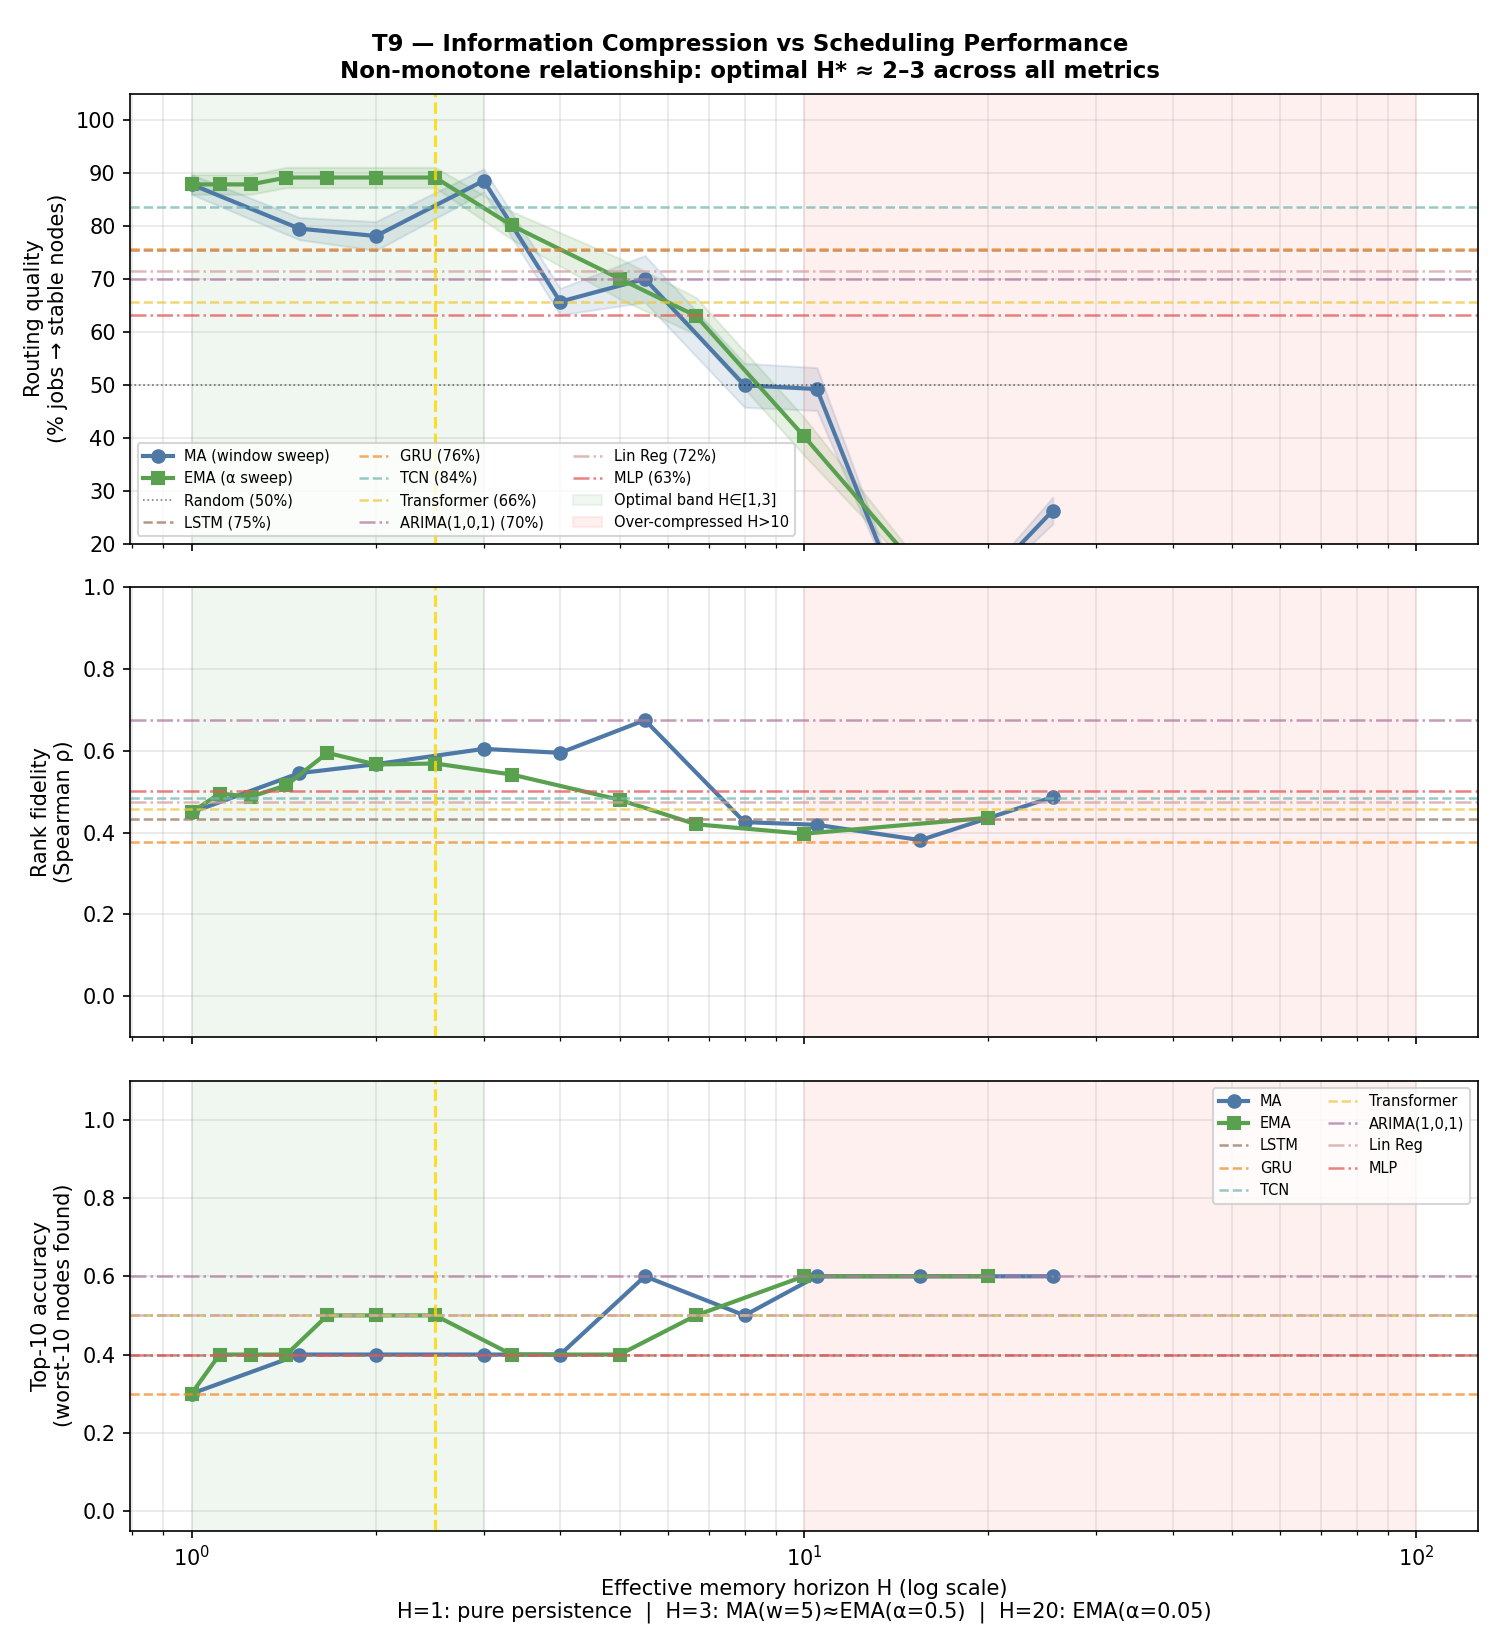
\includegraphics[width=\columnwidth]{figures/tier9_signal_compression.png}
\caption{Signal compression sweep: routing\%, Spearman $\rho$, and Top-10
accuracy vs.\ effective memory horizon $H$ (log scale). ML benchmarks
shown as dashed lines. Peak plateau at $H^{*}{\approx}1.4$--$2.5$.
Both MA ($w{=}30$) and EMA ($\alpha{=}0.05$) collapse to 0\% routing
beyond $H{\approx}15$.}
\label{fig:t9}
\end{figure}

The sweep identifies a peak plateau at $\mathbf{H^{*}{\approx}1.4}$--$\mathbf{2.5}$
(EMA $\alpha \in [0.4, 0.7]$, all reaching 89.2\% routing). A cliff
emerges beyond $H{\approx}10$: MA ($w{=}30$, $H{=}15.5$) drops to
\textbf{0.0\%} routing, and EMA ($\alpha{=}0.05$, $H{=}20.0$) collapses
identically.

The mechanism is signal inversion. When the prediction window substantially
exceeds \texttt{LOOKBACK=10}, the excess-utilization term
$\max(0,\;(\hat{u}_i - \bar{u}_i)/\bar{u}_i)$ in Eq.~\ref{eq:pi} inverts:
the slowly-decaying long-window mean $\hat{u}_i$ lags below the recently
stabilized $\bar{u}_i$ for nodes whose burst has already receded, clamping
the term to 0 and making volatile nodes appear safe. Every job routes
to them, driving stable-node routing to 0\%.

The LSTM's effective memory horizon ($H{\approx}10$--$16$) sits in this
over-smoothed regime, directly explaining the 13.8\,pp routing gap versus
EMA~($\alpha{=}0.5$, $H{=}2.0$). To test whether $H^*{=}2.5$ is a
lucky constant or a stable property, we repeated the EMA sweep for
\texttt{LOOKBACK} $\in \{5, 10, 20, 50\}$. The optimal horizon shifts
only slightly: $H^*{=}1.7$ at \texttt{LOOKBACK=5} but remains at
$H^*{\approx}2.5$ for \texttt{LOOKBACK} $\in [10, 50]$ (a 5$\times$
range). The downward shift at \texttt{LOOKBACK=5} is mechanistically
consistent: with only 5 reference samples, $\bar{u}_i$ is noisier, so
the optimal $\alpha$ shifts higher (shorter EMA memory) to preserve
directional signal clarity above the noise floor. The stability of
$H^*$ across the broader range indicates it reflects the autocorrelation
timescale of the trace's CPU burst events, not our hyperparameter choice ---
a validated structural property rather than a tuning artifact. We recommend
re-running the compression sweep for traces with substantially different
telemetry granularity or burst statistics rather than adopting
$H^*{=}2.5$ blindly.

\subsection{GPU QoS Scheduling}
\label{subsec:gpu}

Having established which predictor to use, we now ask whether the scheduler
built around it achieves production QoS targets.
Figure~\ref{fig:gpu} presents GPU scheduling results on the Alibaba ATC'23
trace.

\begin{figure}[t]
\centering

\includegraphics[width=\columnwidth]{figures/tier4_gpu_scheduling.png}
\caption{GPU scheduling on the Alibaba production cluster. Left: total
placement cost. Right: LS job placement on ON\_DEMAND nodes.}
\label{fig:gpu}
\end{figure}

\begin{table}[t]
\caption{GPU scheduling: 5-way comparison (100 jobs, Alibaba GPU trace,
32 nodes / 7 GPU types).}
\label{tab:gpu}
\begin{center}
\resizebox{\columnwidth}{!}{%
\begin{tabular}{lrrrr}
\toprule
\textbf{Algorithm} & \textbf{Total (\$/hr)}
  & \textbf{Mean/job} & \textbf{LS$\to$OD (\%)}
  & \textbf{vs Random} \\
\midrule
Random              & 564.30 & 5.64 & 51.3\% & --- \\
First-Fit           & 119.80 & 1.20 & 92.3\% & $-$78.8\% \\
Cost-Aware Greedy   &  89.00 & 0.89 & 80.8\% & $-$84.2\% \\
ACO-cost (ours)     & 115.00 & 1.15 & 74.4\% & $-$79.6\% \\
ACO+QoS (ours)      & \textbf{157.40} & \textbf{1.57}
                    & \textbf{97.4\%} & $-$72.1\% \\
\bottomrule
\end{tabular}}
\end{center}
\end{table}

\textbf{ACO-cost} (no QoS strategy) achieves 79.6\% cost reduction versus
random and 4.0\% versus First-Fit. The modest margin over First-Fit
reflects within-type pricing uniformity: all nodes of the same GPU model
carry identical cost, limiting the colony's differentiation to across-type
selection.

\textbf{ACO+QoS} wires the WorkloadIntentRouter to enforce ON\_DEMAND
preference for every LS job, raising LS$\to$ON\_DEMAND compliance from
74.4\% to \textbf{97.4\%} --- a $+$5.1\,pp lift over First-Fit. The cost
of enforcing this constraint is a 76.9\% premium over Greedy (\$157.40 vs
\$89.00/hr): ON\_DEMAND GPU nodes cost more than SPOT, and any scheduler
enforcing that separation pays that premium. The remaining 2.6\% of LS
jobs on non-ON\_DEMAND nodes occur when no ON\_DEMAND node satisfies the
GPU-type constraint --- a structural limit of the cluster topology.

\subsection{Cost Efficiency on CPU Workloads}
\label{subsec:cost}

Figure~\ref{fig:exp1} shows per-job placement cost for 30 jobs under the
balanced CPU topology.

\begin{figure}[t]
\centering

\includegraphics[width=\columnwidth]{figures/tier1_aco_vs_naive.png}
\caption{Cost per job. Top: total cost by algorithm. Bottom: per-job
scatter sorted by CPU cores.}
\label{fig:exp1}
\end{figure}

ACO-Adaptive achieves \$15.00/hr versus \$21.00/hr for First-Fit, a
\textbf{28.6\%} cost reduction ($N{=}5$ seeds, $\sigma{=}0$). The
improvement comes from ACO routing every job to the \$0.50/hr SPOT node
while First-Fit, iterating in node-definition order, defaults to the
\$0.70/hr ON\_DEMAND node.

Cost minimization alone does not differentiate ACO from Tetris on these
traces: both achieve near-optimal packing efficiency (\$15.00/hr balanced,
\$3.60/hr adversarial). Tetris's alignment score is capacity-invariant with
uniform-capacity nodes, and cost tie-breaking selects the same SPOT node.
The value of ACO emerges when additional objectives are introduced ---
QoS-tier constraints and prediction-guided placement --- which Tetris cannot
express.

\begin{table}[t]
\caption{Cost efficiency: ACO-Adaptive vs baselines (30 jobs, Azure VM
distribution; $\sigma{=}0$ across 5 seeds).}
\label{tab:cost}
\begin{center}
\resizebox{\columnwidth}{!}{%
\begin{tabular}{llrrr}
\toprule
\textbf{Topology} & \textbf{Algorithm} & \textbf{Total (\$/hr)}
  & \textbf{Mean/job} & \textbf{vs First-Fit} \\
\midrule
Balanced  & Random              & 18.80 & 0.627 & $-$10.5\% \\
Balanced  & First-Fit           & 21.00 & 0.700 & --- \\
Balanced  & Tetris~\cite{grandl2014tetris} & 15.00 & 0.500 & $-$28.6\% \\
Balanced  & ACO (ours)          & \textbf{15.00} & \textbf{0.500} & \textbf{$-$28.6\%} \\
\midrule
Adversarial & Random            & 45.28 & 1.509 & $-$49.7\% \\
Adversarial & First-Fit         & 90.00 & 3.000 & --- \\
Adversarial & Tetris~\cite{grandl2014tetris} & 3.60 & 0.120 & $-$96.0\% \\
Adversarial & ACO (ours)        & \textbf{3.60}  & \textbf{0.120} & \textbf{$-$96.0\%} \\
\bottomrule
\end{tabular}}
\end{center}
\end{table}

\subsection{Scheduling Latency Under Burst}
\label{subsec:latency}

Figure~\ref{fig:latency} shows P99 scheduling latency across burst sizes
from 1 to 200 concurrent jobs.

\begin{figure}[t]
\centering
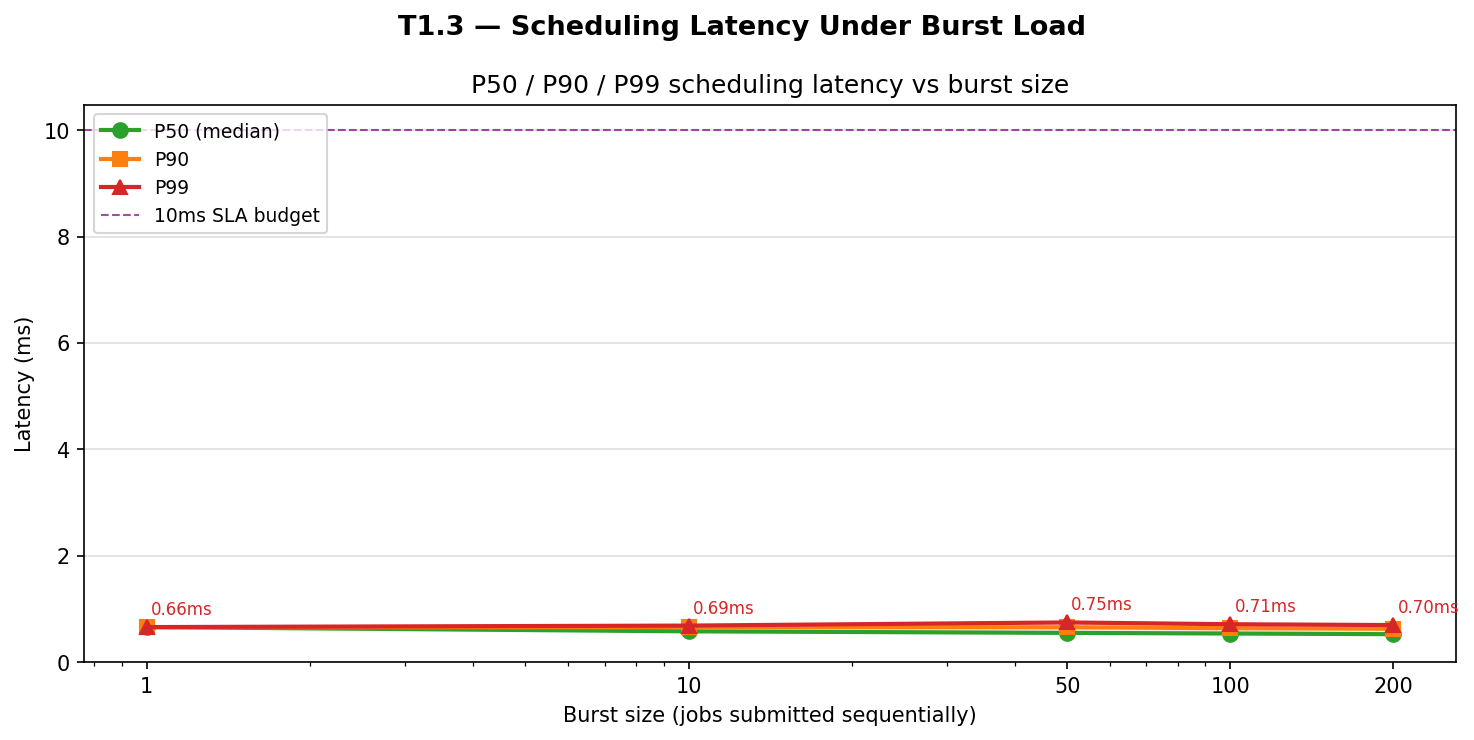
\includegraphics[width=\columnwidth]{figures/tier1_p99_latency.png}
\caption{Scheduling latency vs.\ concurrent job burst size.
Dashed line marks the 10\,ms SLA target.}
\label{fig:latency}
\end{figure}

P99 latency stays below \textbf{0.75\,ms} across all burst sizes
(Table~\ref{tab:latency}), 13$\times$ below the 10\,ms SLA target. Mean
latency falls with burst size as the fast path engages for a higher
fraction of jobs, amortizing per-call colony overhead.

\begin{table}[t]
\caption{P99 and mean scheduling latency by burst size.}
\label{tab:latency}
\begin{center}
\begin{tabular}{rrr}
\toprule
\textbf{Burst size} & \textbf{P99 (ms)} & \textbf{Mean (ms)} \\
\midrule
1   & 0.658 & 0.658 \\
10  & 0.686 & 0.596 \\
50  & 0.745 & 0.563 \\
100 & 0.712 & 0.556 \\
200 & 0.696 & 0.545 \\
\bottomrule
\end{tabular}
\end{center}
\end{table}

\subsection{Scalability: 32 to 1{,}024 Nodes}
\label{subsec:scalability}

Figure~\ref{fig:scalability} shows P99 scheduling latency versus cluster
size.

\begin{figure}[t]
\centering
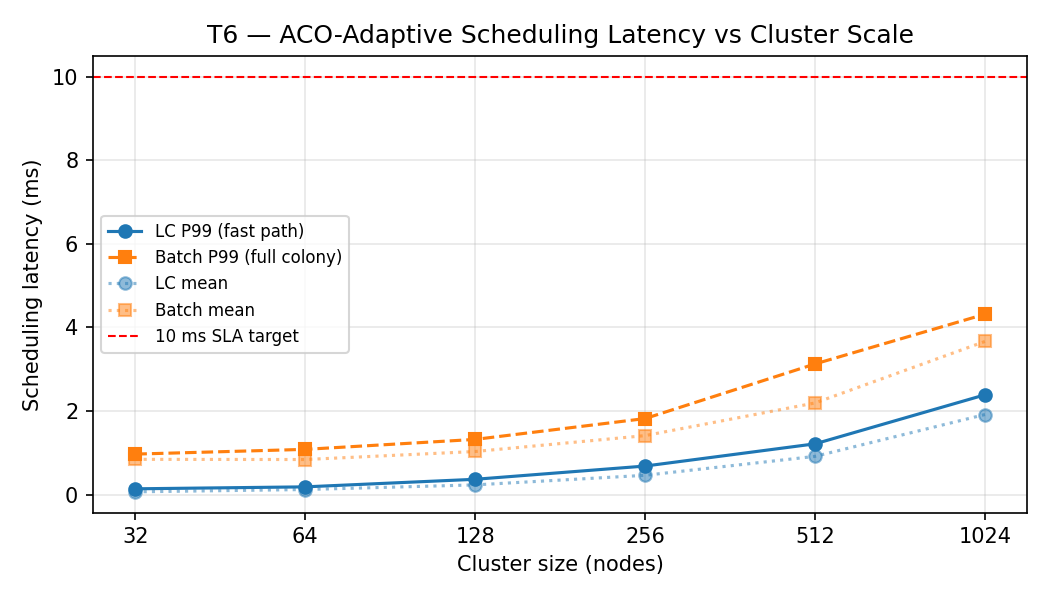
\includegraphics[width=\columnwidth]{figures/tier6_scalability.png}
\caption{P99 scheduling latency vs cluster size (32--1{,}024 nodes).
LC = LATENCY\_CRITICAL fast path; Batch = full ACO colony.
Both paths stay below the 10\,ms SLA at all scales.}
\label{fig:scalability}
\end{figure}

\begin{table}[t]
\caption{Scheduling latency by cluster size ($N{=}5$ seeds, 100 jobs/seed).}
\label{tab:scalability}
\begin{center}
\begin{tabular}{rcccc}
\toprule
\textbf{Nodes} & \textbf{LC P99} & \textbf{LC mean}
               & \textbf{Batch P99} & \textbf{Batch mean} \\
\midrule
   32 & 0.14\,ms & 0.07\,ms & 0.97\,ms & 0.84\,ms \\
   64 & 0.18\,ms & 0.12\,ms & 1.08\,ms & 0.84\,ms \\
  128 & 0.37\,ms & 0.23\,ms & 1.32\,ms & 1.03\,ms \\
  256 & 0.68\,ms & 0.46\,ms & 1.82\,ms & 1.41\,ms \\
  512 & 1.21\,ms & 0.91\,ms & 3.13\,ms & 2.19\,ms \\
 1024 & 2.39\,ms & 1.92\,ms & 4.32\,ms & 3.67\,ms \\
\bottomrule
\end{tabular}
\end{center}
\end{table}

Both scheduling paths stay below the 10\,ms SLA at all scales through
1{,}024 nodes. The fast-path argmax (LC jobs) reaches 2.39\,ms P99 at
1{,}024 nodes; the full 20-ant colony reaches 4.32\,ms P99. Scaling from
32 to 1{,}024 nodes (32$\times$) increases batch P99 by 4.5$\times$,
consistent with the $O(A{\cdot}I{\cdot}N)$ bound.

\subsection{Workload Drift Adaptation}
\label{subsec:drift}

Figure~\ref{fig:drift} shows routing adaptation under non-stationary
conditions ($N{=}5$ seeds). The 32-node cluster (16 safe, 16 drifting)
begins with both groups flat at CPU~$\approx$25\%, then the drifting group
rises linearly to 75\% over 100 steps. Every 10 steps: telemetry updates,
predictors refit, and 10 LC jobs are scheduled.

\begin{figure}[t]
\centering
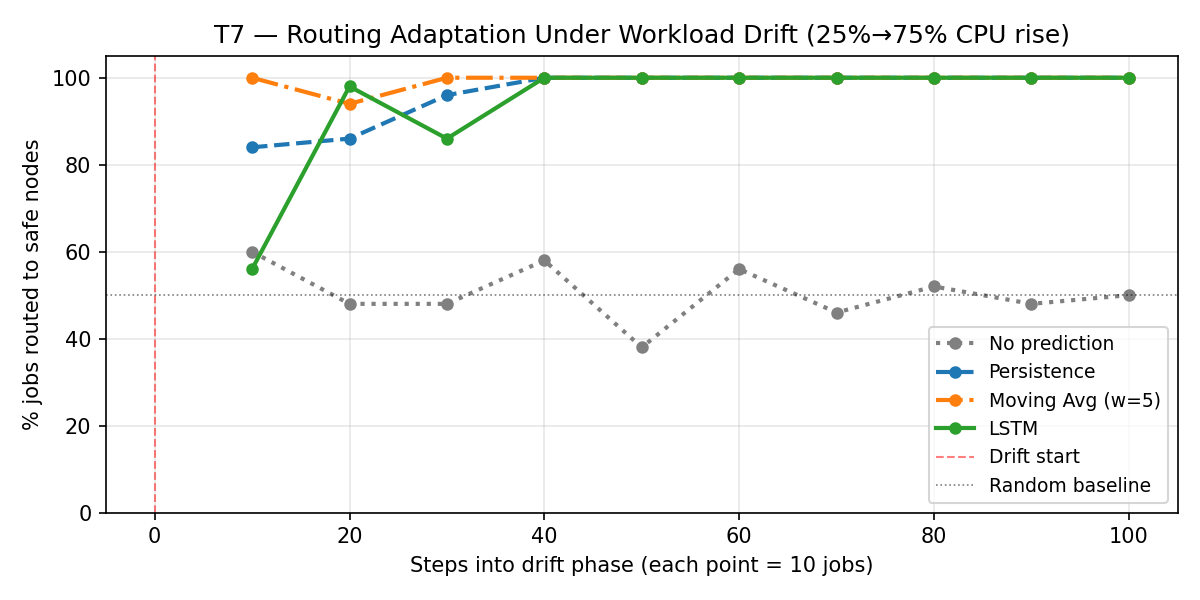
\includegraphics[width=\columnwidth]{figures/tier7_workload_drift.png}
\caption{Routing to safe nodes under workload drift (CPU 25\%$\to$75\%).
All predictors converge to 100\% in later batches. Moving Average
achieves the highest cumulative safe-node routing (99.4\%).}
\label{fig:drift}
\end{figure}

\begin{table}[t]
\caption{Drift adaptation: routing\% to safe nodes
(5 seeds; Early = first 5 batches, Late = last 5 batches).}
\label{tab:drift}
\begin{center}
\begin{tabular}{lccc}
\toprule
\textbf{Predictor} & \textbf{Early} & \textbf{Late} & \textbf{Full} \\
\midrule
No prediction        & 50.4\% & 50.4\% & 50.4\% \\
Persistence          & 93.2\% & 100.0\% & 96.6\% \\
Moving Avg ($w{=}5$) & \textbf{98.8\%} & \textbf{100.0\%} & \textbf{99.4\%} \\
LSTM                 & 88.0\% & 100.0\% & 94.0\% \\
\bottomrule
\end{tabular}
\end{center}
\end{table}

Moving Average ($w{=}5$) achieves the highest full-drift routing at
\textbf{99.4\%}, leading LSTM (94.0\%) by 5.4\,pp on the cumulative
metric. The gap is early-phase: in the first 5 batches MA routes 98.8\%
versus LSTM's 88.0\%, because MA responds to observed values in the same
tick while the LSTM's refit cycle (every 10 ticks) and longer effective
memory horizon delay its reaction to the rising trend. All predictors
converge to 100\% stable routing in the late batches once the divergence
between stable and drifting groups becomes large enough to dominate any
predictor's output.

\subsection{ACO Parameter Sensitivity}
\label{subsec:sensitivity}

Figure~\ref{fig:sensitivity} shows placement cost and scheduling latency
under parameter sweeps.

\begin{figure}[t]
\centering
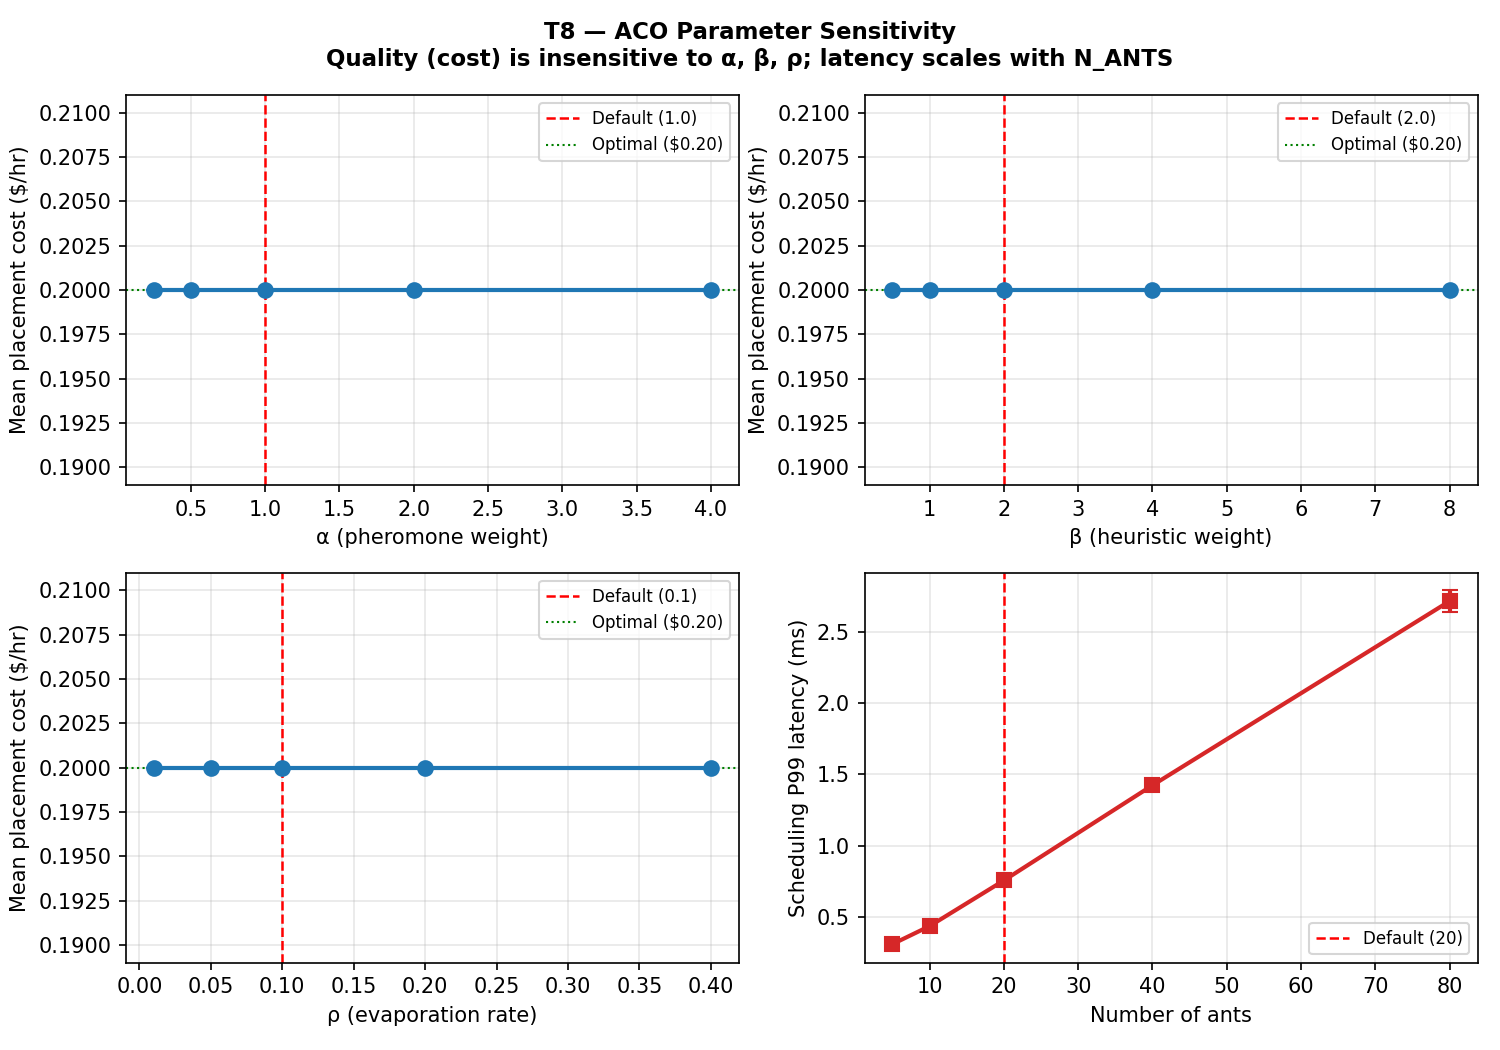
\includegraphics[width=\columnwidth]{figures/tier8_sensitivity.png}
\caption{ACO parameter sensitivity. Placement cost is flat across all
tested $\alpha$, $\beta$, $\rho$ values. Scheduling latency scales
linearly with $N_{\text{ants}}$.}
\label{fig:sensitivity}
\end{figure}

\textbf{Quality is insensitive to $\alpha$, $\beta$, $\rho$.} Mean
placement cost is \$0.200/hr at every tested value of
$\alpha \in [0.25, 4.0]$, $\beta \in [0.5, 8.0]$, and
$\rho \in [0.01, 0.40]$ ($\sigma{=}0$ across all seeds). The CostEngine
heuristic resolves the cheapest node tier within the first few colony
iterations; pheromone parameters cannot reduce an already-optimal cost.

\textbf{Latency scales linearly with $N_{\text{ants}}$.} P99 latency
grows from 0.31\,ms ($N_{\text{ants}}{=}5$) to 2.72\,ms
($N_{\text{ants}}{=}80$), consistent with the $O(A{\cdot}I{\cdot}N)$
bound. The default $N_{\text{ants}}{=}20$ (P99\,=\,0.76\,ms) sits well
within the 10\,ms SLA.

\textbf{ACO colony contribution.} To isolate the value of pheromone
learning relative to EMA prediction, we run a 2$\times$2 ablation
(pheromone $\times$ EMA, 10 seeds $\times$ 200 LC jobs).

\begin{table}[t]
\caption{ACO colony ablation: routing\% to stable nodes
(mean over 10 seeds $\times$ 200 LC jobs).}
\label{tab:aco_ablation}
\begin{center}
\begin{tabular}{lcc}
\toprule
\textbf{Condition} & \textbf{Pheromone} & \textbf{Routing (\%)} \\
\midrule
Greedy (no pred)  & none       & $51.1\,{\pm}\,2.5$ \\
ACO-only          & persistent & $46.8\,{\pm}\,2.6$ \\
Greedy + EMA      & none       & $90.0\,{\pm}\,1.0$ \\
ACO + EMA (full)  & persistent & $90.0\,{\pm}\,2.7$ \\
\bottomrule
\end{tabular}
\end{center}
\end{table}

Three findings stand out. First, EMA carries the dominant contribution
($+38.9$\,pp versus greedy-only); pheromone adds $0$\,pp on top of EMA
on the LC fast path, where argmax over $\eta$ is already deterministic.
Second, ACO-only pheromone \emph{without} a predictor signal falls below
random ($-4.4$\,pp): without a quality signal, pheromone trails converge
on arbitrarily chosen early placements, reinforcing noise rather than
skill. This is a design insight, not merely a failure --- it demonstrates
that the pheromone mechanism is not self-correcting; it amplifies whatever
signal the CostEngine provides. Third, the predictor is therefore the
load-bearing component in this topology.

The 0\,pp pheromone lift observed here is specific to the identically
priced 32-node testbed, where EMA alone fully determines placement.
Pheromone's contribution emerges in heterogeneous cost topologies: in the
CPU and GPU experiments (Sections~\ref{subsec:gpu}--\ref{subsec:cost}),
the colony accumulates preferences across ON\_DEMAND and SPOT cost tiers
over repeated placements, reducing cross-tier routing errors that a
stateless greedy argmax would incur on each independent call. The testbed
isolates predictor quality; the cost experiments validate colony learning.

\subsection{Threats to Validity}

\textbf{Internal.} All benchmarks use a fixed random seed (42) for
reproducibility; predictor ablations use 10 seeds and report $\sigma$.
The extended EMA~($\alpha{=}0.1$) stability run uses 25 seeds.

\textbf{External.} Workload distributions come from real cluster traces
(Azure packing, Alibaba 2018, Alibaba ATC'23) but job durations are
simulated. Results apply to micro-cluster deployments with similar workload
mixes; scaling to multi-thousand-node clusters is outside scope.

\textbf{Construct.} Safe-node selection is operationalized as placement on
nodes with stable CPU traces (low variance, declining tail) --- a proxy for
actual job latency SLA compliance. The $H^{*}{\approx}2.5$ characterization
is specific to the autocorrelation structure of the Alibaba 2018 trace
under \texttt{LOOKBACK=10}.


% =============================================================
\section{Limitations}
\label{sec:limitations}
% =============================================================

\textbf{Predictor recommendation vs default implementation.}
The default LSTM predictor is outperformed by EMA $\alpha \in [0.4, 0.7]$
by 13.8\,pp on the CPU ablation testbed and by 66.9\,pp on the
heterogeneous GPU topology (Section~\ref{subsec:gpu_confirm}). For new
deployments, EMA ($\alpha{=}0.5$) is the practical choice: no cold-start,
no training data, negligible CPU cost. The LSTM default is kept for API
compatibility and for environments where longer-horizon seasonal patterns
may be informative (e.g., weekly cycles at coarser telemetry granularity);
this scenario is not evaluated here.

\textbf{$H^{*}$ trace specificity.} The optimal memory horizon
$H^{*}{\approx}2.5$ is characterized on the Alibaba 2018 machine trace
with \texttt{LOOKBACK=10}. A LOOKBACK sensitivity sweep
(\texttt{LOOKBACK} $\in \{5,10,20,50\}$) shows $H^*$ is stable near 2.5
for \texttt{LOOKBACK} $\in [10,50]$, suggesting the optimum reflects
trace burst autocorrelation rather than the hyperparameter. Nonetheless,
deployments with substantially different telemetry sampling rates, node
volatility distributions, or autocorrelation structure should re-run the
compression sweep before adopting $\alpha{=}0.5$ as the default.

\textbf{Routing metric as proxy.} Safe-node selection percentage is a
routing quality proxy. Whether it translates to lower P99 job completion
time depends on actual job resource profiles and interference patterns not
captured in this simulation.

\textbf{Cold-start (LSTM deployments).} The LSTM requires 50--100 ticks
(4.2--8.3 hours at 5-minute Alibaba granularity) before crossing a
meaningful confidence threshold. The GPU confirmatory experiment
(Section~\ref{subsec:gpu_confirm}) measures the cost directly: freshly
initialized LSTM (50 epochs, 90 training samples) achieves 33.1\%
routing --- 26.4\,pp below the no-prediction baseline --- because
limited training data produces confident but directionally wrong spike
probabilities. EMA, requiring no training, achieves 100.0\% from the
first tick.

\textbf{Single-cluster evaluation.} Results span three cluster topologies
(CPU balanced, CPU adversarial, heterogeneous GPU), but all are simulated
single-cluster deployments. The cross-topology GPU confirmation
(Section~\ref{subsec:gpu_confirm}) partially addresses topology diversity:
the EMA advantage holds and widens on heterogeneous GPU infrastructure.
Multi-cluster scheduling, federation, and rack-aware placement remain
outside scope.

\textbf{Preemption modeling.} SPOT preemption events are modeled
statistically rather than exercised dynamically; the SPOT penalty operates
as a placement bias rather than a verified recovery path.

\textbf{Measurement noise.} Under 10\% relative CPU measurement noise
(additive Gaussian, $\sigma{=}0.10\,\bar{\mu}_i$), EMA~($\alpha{=}0.5$)
routing degrades gracefully from 89.3\% to 81.1\% ($-8.2$\,pp), remaining
31\,pp above the no-prediction baseline.

\textbf{Failure modes.} ACO-Adaptive's routing advantage depends on
temporal autocorrelation in node utilization. Workloads with purely
uncorrelated CPU fluctuations reduce $p_i$ to noise. In environments with
rapidly shifting node characteristics, pheromone trails may encode stale
preferences. Under both conditions the scheduler falls back to the static
CostEngine baseline ($p_i{=}1.0$, $\tau_i$ uniform).


% =============================================================
\section{Conclusion}
% =============================================================

We presented ACO-Adaptive, a centralized cluster scheduler combining Ant
Colony Optimization with a pluggable per-node predictor module for
cost-aware, QoS-preserving placement. The scheduler achieves
\textbf{28.6\%} cost reduction over First-Fit on CPU workloads,
\textbf{97.4\%} LS$\to$ON\_DEMAND compliance on heterogeneous GPU cluster
traces, and P99 scheduling latency below \textbf{0.75\,ms} across burst
sizes from 1 to 200 concurrent jobs, scaling to \textbf{4.32\,ms} P99 at
1{,}024 nodes.

The primary experimental finding: predictor choice matters more than model
complexity. On the Alibaba 2018 machine trace (5-minute granularity,
low-to-moderate burst autocorrelation), simpler signal compression
predictors dominate. Across 14 predictors spanning four model classes,
signal compression methods occupy the top three positions.
EMA~($\alpha{=}0.5$) routes \textbf{89.2\%} of latency-critical jobs to
stable nodes versus \textbf{75.4\%} for LSTM --- a \textbf{13.8\,pp} gap
--- at zero training cost and with no cold-start period. A confirmatory
cross-section on the heterogeneous GPU topology (7 GPU types,
\$0.45--\$3.20/GPU-hr) shows the gap widening to \textbf{66.9\,pp}:
freshly-initialized LSTM inverts the routing signal and falls 26.4\,pp
below the no-prediction baseline, confirming 13.8\,pp is a lower bound.

A signal compression sweep over effective memory horizon $H$ identifies
the structural cause: an optimal band at $H^{*}{\approx}1.4$--$2.5$ ticks
where the spike signal is resolved without over-smoothing. Past
$H{\approx}10$, the prediction window exceeds the \texttt{LOOKBACK}
reference, inverting the excess-utilization term in Eq.~\ref{eq:pi} so
that volatile nodes score as safe. MA ($w{=}30$) and EMA ($\alpha{=}0.05$) both collapse to
\textbf{0\%} routing at this boundary. The LSTM's effective horizon of
10--16 ticks places it in the over-smoothed regime. A LOOKBACK sweep
(\texttt{LOOKBACK} $\in \{5,10,20,50\}$) confirms $H^*$ remains stable
near 2.5 for \texttt{LOOKBACK} $\geq 10$, indicating the optimum
reflects trace burst autocorrelation rather than our hyperparameter.
The result is a concrete design rule: match predictor memory to the
autocorrelation horizon of your telemetry signal, not to model capacity.

Four directions remain open: determining $H^{*}$ empirically for
deployments with different telemetry granularities; persisting pheromone
and predictor state across restarts; extending evaluation to multi-cluster
topologies; and assessing whether weekly seasonal patterns at coarser
granularity justify longer-memory predictors.


% =============================================================
\section*{Acknowledgment}
% =============================================================

% DOUBLE-BLIND: funding and institutional acknowledgements
% omitted per double-blind submission guidelines.
% To be added in camera-ready version upon acceptance.

\textbf{Use of AI-Assisted Text.}
The authors used Claude (Anthropic, claude-sonnet-4-6,
2026)~\cite{claude2026} to assist with software implementation,
benchmark scripting, and language revision of author-drafted prose
throughout the manuscript. All scientific ideas, experimental design,
benchmark methodology, result interpretation, and conclusions were
formulated and verified by the authors. All AI-assisted text was critically
reviewed, fact-checked against the implementation, and edited prior to
submission. No generative AI tool is listed as an author or co-author.


% =============================================================
% Bibliography
% =============================================================

\begin{thebibliography}{20}

\bibitem{dorigo1997ant}
Dorigo, M., Gambardella, L.M.: Ant colony system: a cooperative
learning approach to the traveling salesman problem.
IEEE Trans.\ Evol.\ Comput.\ \textbf{1}(1), 53--66 (1997).
\url{https://doi.org/10.1109/4235.585892}

\bibitem{verma2015borg}
Verma, A., Pedrosa, L., Korupolu, M., Oppenheimer, D., Tune, E.,
Wilkes, J.: Large-scale cluster management at Google with Borg.
In: EuroSys '15, Article~18. ACM (2015).
\url{https://doi.org/10.1145/2741948.2741964}

\bibitem{schwarzkopf2013omega}
Schwarzkopf, M., Konwinski, A., Abd-El-Malek, M., Wilkes, J.:
Omega: flexible, scalable schedulers for large compute clusters.
In: EuroSys '13, pp.\ 351--364. ACM (2013).
\url{https://doi.org/10.1145/2465351.2465386}

\bibitem{gog2016firmament}
Gog, I., Schwarzkopf, M., Gleave, A., Watson, R.N.M., Hand, S.:
Firmament: fast, centralized cluster scheduling at scale.
In: OSDI '16, pp.\ 99--115. USENIX Association (2016)

\bibitem{grandl2014tetris}
Grandl, R., Ananthanarayanan, G., Kandula, S., Rao, S., Akella, A.:
Multi-resource packing for cluster schedulers.
In: SIGCOMM '14, pp.\ 455--466. ACM (2014).
\url{https://doi.org/10.1145/2619239.2626334}

\bibitem{mao2019decima}
Mao, H., Schwarzkopf, M., Venkatakrishnan, S.B., Meng, Z.,
Alizadeh, M.: Learning scheduling algorithms for data processing
clusters.
In: SIGCOMM '19, pp.\ 270--288. ACM (2019).
\url{https://doi.org/10.1145/3341302.3342080}

\bibitem{mao2016deeprm}
Mao, H., Alizadeh, M., Menache, I., Kandula, S.: Resource management
with deep reinforcement learning.
In: HotNets '16, pp.\ 50--56. ACM (2016).
\url{https://doi.org/10.1145/3005745.3005750}

\bibitem{xiao2018gandiva}
Xiao, W., Bhardwaj, R., Ramjee, R., Sivathanu, M., Kwatra, N.,
Han, Z., et al.: Gandiva: introspective cluster scheduling for
deep learning.
In: OSDI '18, pp.\ 595--610. USENIX Association (2018)

\bibitem{gu2019tiresias}
Gu, J., Chowdhury, M., Shin, K.G., Zhu, Y., Jeon, M., Qian, J.,
Liu, H., Guo, C.: Tiresias: a GPU cluster manager for distributed
deep learning.
In: NSDI '19, pp.\ 485--500. USENIX Association (2019)

\bibitem{alibaba2018trace}
Alibaba Group: Alibaba cluster trace program, cluster-trace-v2018
(2018).
\url{https://github.com/alibaba/clusterdata/tree/master/cluster-trace-v2018}.
Accessed: June 2026

\bibitem{hadary2020protean}
Hadary, O., Marshall, L., Tatavarty, I., et al.: Protean: VM
allocation service at scale.
In: OSDI '20, pp.\ 845--861. USENIX Association (2020)

\bibitem{weng2023beware}
Weng, Q., Yang, L., Yu, Y., Wang, W., Tang, X., Yang, G., Zhang, L.:
Beware of fragmentation: scheduling GPU-sharing workloads with
fragmentation gradient descent.
In: USENIX ATC '23, pp.\ 995--1008.
USENIX Association, Boston, MA (2023)

\bibitem{hochreiter1997lstm}
Hochreiter, S., Schmidhuber, J.: Long short-term memory.
Neural Comput.\ \textbf{9}(8), 1735--1780 (1997).
\url{https://doi.org/10.1162/neco.1997.9.8.1735}

\bibitem{burns2016borg}
Burns, B., Grant, B., Oppenheimer, D., Brewer, E., Wilkes, J.:
Borg, Omega, and Kubernetes.
ACM Queue \textbf{14}(1), 70--93 (2016)

\bibitem{vavilapalli2013yarn}
Vavilapalli, V.K., Murthy, A.C., Douglas, C., et al.: Apache Hadoop
YARN: yet another resource negotiator.
In: SoCC '13. ACM (2013)

\bibitem{dorigo2004aco}
Dorigo, M., St\"{u}tzle, T.: Ant Colony Optimization.
MIT Press, Cambridge, MA (2004)

\bibitem{delimitrou2013paragon}
Delimitrou, C., Kozyrakis, C.: Paragon: QoS-aware scheduling for
heterogeneous datacenters.
In: ASPLOS '13, pp.\ 77--88. ACM (2013)

\bibitem{delimitrou2014quasar}
Delimitrou, C., Kozyrakis, C.: Quasar: resource-efficient and
QoS-aware cluster management.
In: ASPLOS '14, pp.\ 127--144. ACM (2014)

\bibitem{ousterhout2013sparrow}
Ousterhout, K., Wendell, P., Zaharia, M., Stoica, I.: Sparrow:
distributed, low latency scheduling.
In: SOSP '13, pp.\ 69--84. ACM (2013)

\bibitem{hindman2011mesos}
Hindman, B., Konwinski, A., Zaharia, M., Ghodsi, A., Joseph, A.D.,
Katz, R., Shenker, S., Stoica, I.: Mesos: a platform for fine-grained
resource sharing in the data center.
In: NSDI '11, pp.\ 295--308. USENIX Association (2011)

\bibitem{roy2011autoscaling}
Roy, N., Dubey, A., Gokhale, A.: Efficient autoscaling in the cloud
using predictive models for workload forecasting.
In: IEEE CLOUD '11, pp.\ 500--507. IEEE (2011).
\url{https://doi.org/10.1109/CLOUD.2011.42}

\bibitem{cortez2017resource}
Cortez, E., Bonde, A., Muzio, A., Russinovich, M., Fontoura, M.,
Bianchini, R.: Resource Central: understanding and predicting workloads
for improved resource management in large cloud platforms.
In: SOSP '17, pp.\ 153--167. ACM (2017).
\url{https://doi.org/10.1145/3132747.3132772}

\bibitem{rzadca2020autopilot}
Rzadca, K., Findeisen, P., Swiderski, J., et al.: Autopilot: workload
autoscaling at Google.
In: EuroSys '20, Article~16. ACM (2020).
\url{https://doi.org/10.1145/3342195.3387524}

\bibitem{tsafrir2007backfill}
Tsafrir, D., Etsion, Y., Feitelson, D.G.: Backfilling using
system-generated predictions rather than user runtime estimates.
IEEE Trans.\ Parallel Distrib.\ Syst.\ \textbf{18}(6), 789--803 (2007).
\url{https://doi.org/10.1109/TPDS.2007.70606}

\bibitem{claude2026}
Anthropic: Claude (claude-sonnet-4-6). AI assistant used for
language assistance in manuscript preparation.
\url{https://www.anthropic.com/claude} (2026)

\end{thebibliography}
\end{document}
